\documentclass[11pt]{article} % use larger type; default would be 10pt

%\usepackage[utf8]{inputenc} % set input encoding (not needed with XeLaTeX)
\usepackage[parfill]{parskip}
%%%% PAGE DIMENSIONS
\usepackage{geometry} 
\geometry{a4paper} % or letterpaper (US) or a5paper or\cdots\cdots
\geometry{margin=0.6in} % for example, change the margins to 2 inches all round
%
\usepackage{graphicx} % support the \includegraphics command and options
%\usepackage[parfill]{parskip} % Activate to begin paragraphs with an empty line rather than an indent
%
%%%% PACKAGES
%\usepackage{booktabs} % for much better looking tables
%\usepackage{xfrac}
\usepackage{csquotes}
\usepackage{listings}
%\usepackage{subfigure}
\usepackage{ulem}
\usepackage{amsmath}
\usepackage{amssymb}
%
%% These packages are all incorporated in the memoir class to one degree or another\cdots.
%
%
%%%% HEADERS & FOOTERS
%\usepackage{fancyhdr} % This should be set AFTER setting up the page geometry
%\pagestyle{fancy} % options: empty , plain , fancy
%\renewcommand{\headrulewidth}{0.4pt} % customise the layout\cdots.
%\lhead{}\chead{\footnotesize \textit{IBM Confidential}}\rhead{}
%\lfoot{}\cfoot{\thepage}\rfoot{}
%
%%%% SECTION TITLE APPEARANCE
%\usepackage{sectsty}
%%\allsectionsfont{\sffamily\mdseries\upshape} % (See the fntguide.pdf for font help)
%% (This matches ConTeXt defaults)
%
%
%%COLOURING 
%\usepackage{color}
%\newcommand{\new}{\textcolor{red}}
%%\input{rgb}
%
%%%% ToC (table of contents) APPEARANCE
%\usepackage[nottoc,notlof,notlot]{tocbibind} % Put the bibliography in the ToC
%\usepackage[titles,subfigure]{tocloft} % Alter the style of the Table of Contents
%\renewcommand{\cftsecfont}{\rmfamily\mdseries\upshape}
%\renewcommand{\cftsecpagefont}{\rmfamily\mdseries\upshape} % No bold!
%\usepackage{parskip}
%%%% END Article customizations
%
%%%% The "real" document content comes below\cdots.
%
\title{House Price Machine Learning Homework}
\author{Cecilia Aas}
%\date{20$^{\text{th}}$ October 2015} % Activate to display a given date or no date (if empty),
%         % otherwise the current date is printed 

%
%\def\layersep{\item5cm}
%\setlength{\parindent}{0pt}
\begin{document}
\lstset{language=Python, frame=lines}

\section*{House Prices Machine Learning Homework}
\subsection*{Cecilia Aas}

%The task is to predict the price a property is sold for, based \textit{only} on
%\begin{itemize}
%\item type of duration (freehold, leasehold or other)
%\item type of property (detached, semi-detached, flat/maisonette, or other
%\item whether or not the property is located in London
%\end{itemize}


In this problem, the target variable (price) is continuous while the features (property type, duration, location) are discrete.  Therefore, any model trained on this data can only ever yield a discrete set of possible predictions.\footnote{At most, there can be $N$ possible prediction values, where $N$ is the number of unique feature value combinations.}  My model of choice is random forest regression as this is an efficient and often well-performing approach to predicting continuous target variables from discrete-valued features.\footnote{A random forest consists of a number of decision trees.  Each decision tree in the forest is grown (trained) using a random subset of the training data.  Each node in each tree is split into child nodes so as to minimise the mean-squared error of the training samples filtered through to each child.  This continues until nodes can no longer be split, e.g., because we have limited the number of samples required for splitting (for regularisation purposes), or because there is no feature that can distinguish between the training samples at the node.  Each leaf node represents a particular prediction value, calculated from an average across the labels of the training samples that filtered through to this particular leaf.  This prediction will be the prediction of that decision tree on every test datum that filters through to that leaf.  The final prediction of the random forest for a given test datum is the result of a vote on predictions amongst all the decision trees.}  The parameters for a random forest (e.g., number of trees, maximum depth of each tree, etc.) are normally set by performing grid-search, optimising model performance across parameter space.  Because the instructions explicitly state that we are more interested in the evaluation rather than the performance of the model, I have only done a very rough parameter optimisation for now. Using the parameters given in the code, the root-mean-squared-error of our trained random forest on the test set is approximately \pounds 820 000; this is a huge error, especially considering the standard deviation of the actual test set prices is around \pounds 850 000.  The plot of residuals\footnote{The residual for a given datapoint is defined as the difference between the prediction and the actual value; a positive residual represents an underestimation, and vice versa.} vs predictions (Fig.~1) has a columnar appearance due to there being only a discrete set of possible predictions (as discussed above). The plot is also unbalanced; for the test set (i.e., for property sold in 2015) the underestimations are generally much larger than the overestimations.  This is probably partly an effect of ignoring time (date of purchase) in our model.  By ignoring time in training our model we have effectively averaged out (across the dataset) any temporal effects in our predictions.  Unfortunately for us, house prices have increased significantly with time from 1995 to 2015.  Therefore, training a  house price model while ignoring time will generally underestimate prices from more recent years, and overestimate prices from earlier years.  \textbf{The coefficient of determination ($R^2$ value) for the test set is around 8 \%, meaning only 8 \% of the variance in 2015 house prices can be explained by our model.}  This is not too dissimilar from the $R^2$ value on the training set, 12 \%, meaning there is some degree of overfitting to the training data but in no way an unacceptable amount.  In summary, this model can predict about 8 \% of the variance in 2015 house prices, however, its performance could probably be greatly improved by including time as a variable (although we would need to be careful as we would be extrapolating a model trained on 1995-2014 data to 2015 data).

\begin{figure}
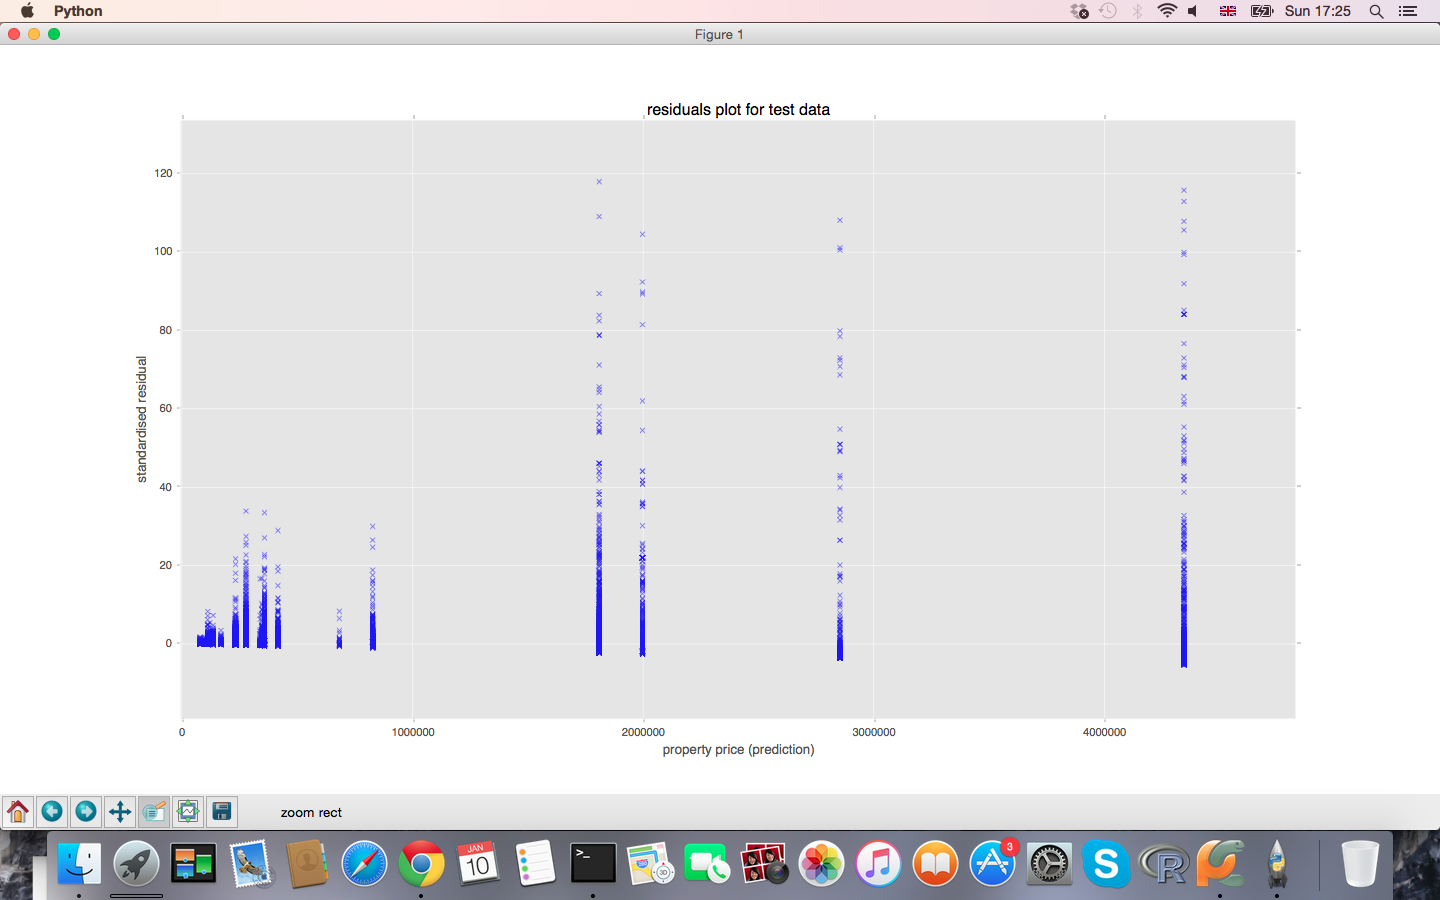
\includegraphics[scale=0.4,trim=30mm 45mm 30mm 35mm, clip]{residuals.png}
\caption{The standardised residuals as a function of predicted price.\label{fig:fige}}
\end{figure}

\end{document}